\section{Performance Metrics}

\begin{table}[h!]
    \begin{center}
        \begin{tabular}{|c|c|c|c|c|c|c|c|}
            \hline
            \multirow{2}{*}{\textbf{Model}} & \multicolumn{3}{|c|}{\textbf{Macro}} & \multicolumn{3}{|c|}{\textbf{Micro}} &  \multirow{2}{*}{\textbf{Accuracy}}\\
            \cline{2-7}
            & \textbf{P} & \textbf{R} & \textbf{F} & \textbf{P} & \textbf{R} & \textbf{F} & \\
            \hline
            Main Model & 0.6500 & 0.6532 & 0.6511 & 0.6557 & 0.6557 & 0.6557 & 65.57\% \\
            \hline
            Variant 1 & 0.6084 & 0.6114 & 0.6077 & 0.6108 & 0.6108 & 0.6108 & 61.08\% \\
            \hline
            Variant 2 & 0.6592 & 0.6412 & 0.6416 & 0.6392 & 0.6392 & 0.6392 &  63.92\% \\
            \hline
        \end{tabular}
        \caption{Comparison of Models}
        \label{tab:model-comparison}
    \end{center}
\end{table}

    \subsection*{Main Model vs Variant 1}
    \begin{itemize}
        \item The Main Model outperforms Variant 1 in terms of accuracy and all macro metrics.
        \item It has a higher overall correctness and a better balance between precision and recall across all classes.
    \end{itemize}

    \subsection*{Main Model vs Variant 2}
    \begin{itemize}
        \item The Main Model has a slightly higher accuracy compared to Variant 2
        \item Variant 2 has a higher macro precision, indicating that it performs better in terms of avoiding false positives.
    \end{itemize}

    \vspace*{1em}

    \noindent If a model has higher recall but lower precision, it tends to capture more relevant instances but at the cost of including more false positives. In facial image analysis, higher recall implies that the model is good at identifying an instances of a particular class. However, lower precision means that there might be more false alarms or misclassifications. \cite{apc}


\section{Confusion Matrix Analysis}

\begin{figure}[h!]
    \centering
  
    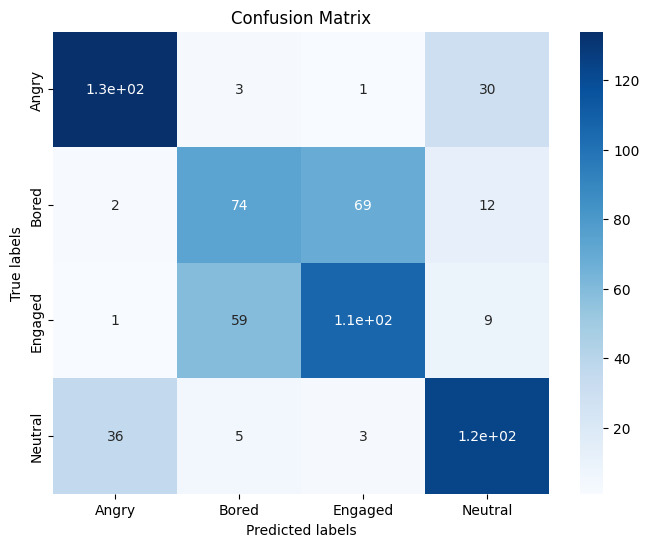
\includegraphics[width=0.3\textwidth, height=5cm]{resources/cfmt-main.jpeg}
    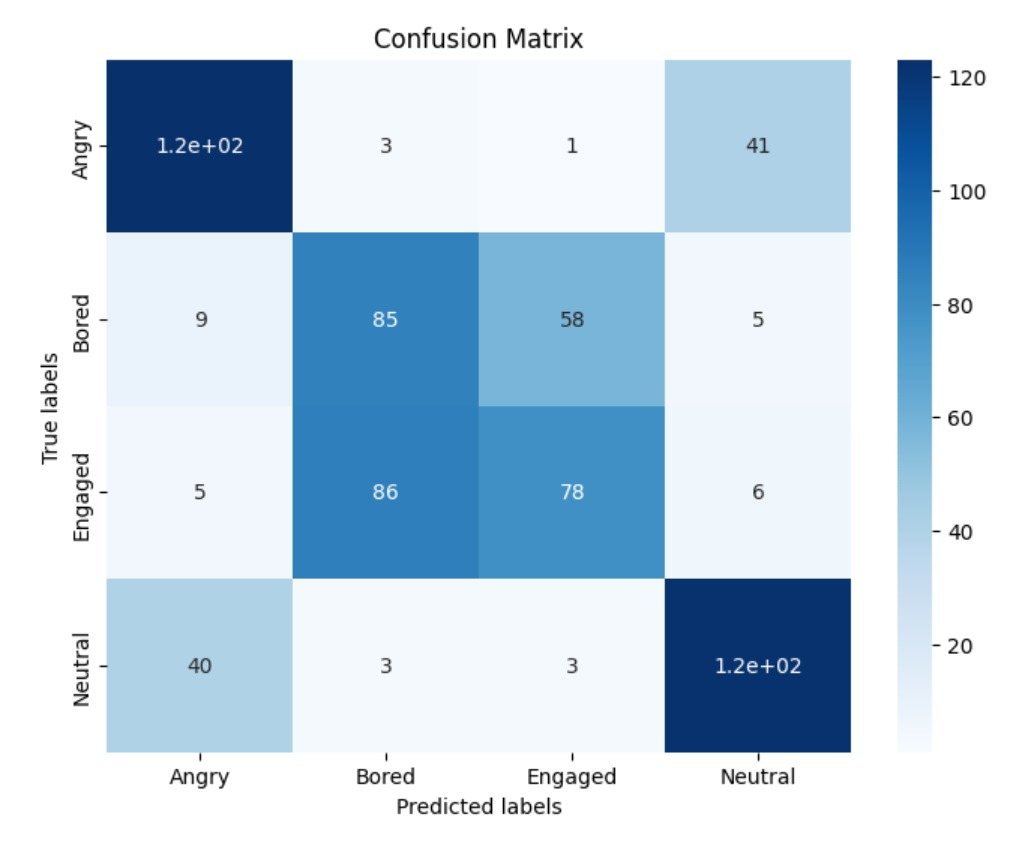
\includegraphics[width=0.3\textwidth, height=5cm]{resources/cfmt-v1.jpeg}
    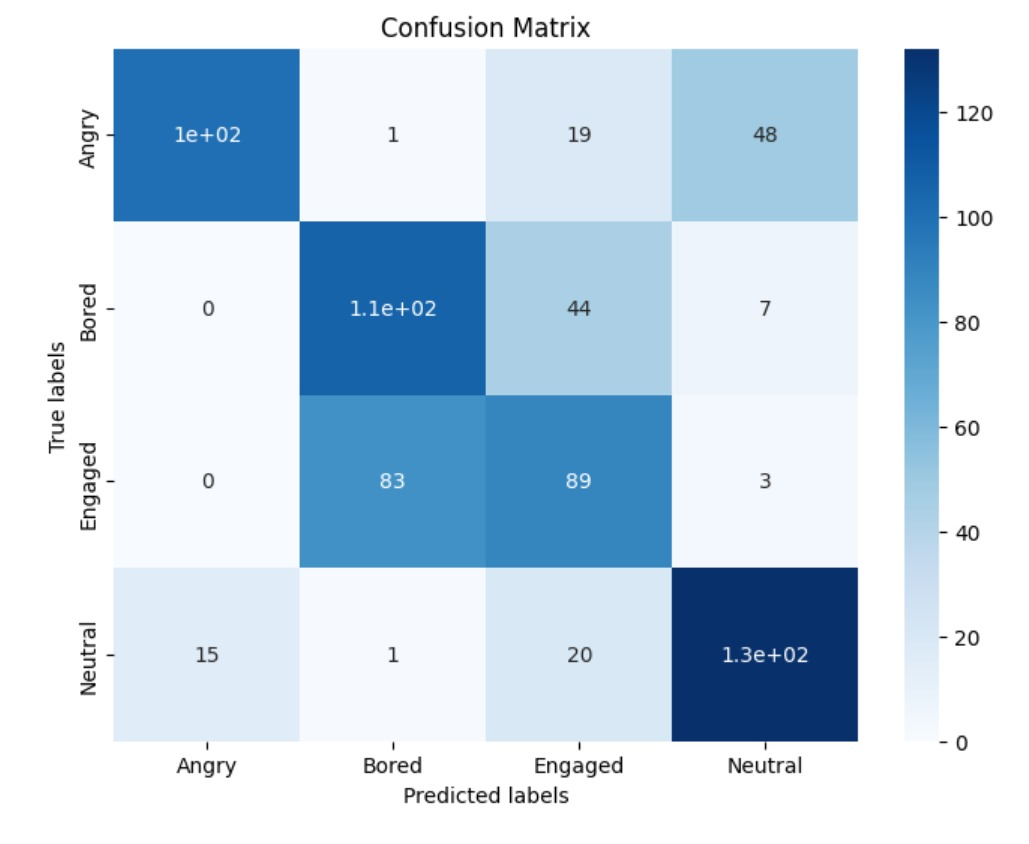
\includegraphics[width=0.3\textwidth, height=5cm]{resources/cfmt-v2.jpeg}

    \centering
    \begin{subfigure}{.3\textwidth}
      \centering
      \[
      \begin{bmatrix}
        130 & 3 & 1 & 30 \\
        2 & 74 & 69 & 12 \\
        1 & 59 & 110 & 9 \\
        36 & 5 & 3 & 120 \\
      \end{bmatrix}
      \]
      \caption{Main Model}
    \end{subfigure}%
    \begin{subfigure}{.3\textwidth}
      \centering
      \[
      \begin{bmatrix}
        120 & 3 & 1 & 41 \\
        9 & 85 & 58 & 5 \\
        5 & 86 & 78 & 6 \\
        40 & 3 & 3 & 120 \\
      \end{bmatrix}
      \]
      \caption{Variant 1}
    \end{subfigure}%
    \begin{subfigure}{.3\textwidth}
      \centering
      \[
      \begin{bmatrix}
        100 & 1 & 19 & 48 \\
        0 & 110 & 44 & 7 \\
        0 & 83 & 89 & 3 \\
        15 & 1 & 20 & 130 \\
      \end{bmatrix}
      \]
      \caption{Variant 2}
    \end{subfigure}
    \caption{Confusion Matrices for Main Model, Variant 1, and Variant 2}
  \end{figure}

  \begin{itemize}
    \item Main Model - Class 2 (Bored) is often confused with Class 3 (Engaged). This is observed from the significant value in the (1, 2) cell.
    \item Variant 1 \& 2 - Similar patterns of confusion as the Main Model, with Class 3 (Engaged) and Class 2 (Bored) having notable misclassifications.
    \item There's a consistent trend across models where Engaged (Class 3) and Bored (Class 2) are often confused. This could be due to similarities in facial expressions or insufficient distinguishing features.
    \item The Neutral and Angry classes seem to be well-recognized across all models, suggesting that these facial expressions are more consistent and universally recognizable.
    \item Overall, distinguishing between expressions Class 3 (Engaged) and Class 2 (Bored) poses a challenge for these models. This might be due to the lack of diversity and quality of data.
\end{itemize}
\section{Impact of Architectural Variations}
\noindent Increasing the depth (number of convolutional layers) from the main model to Variant 2 did not consistently improve performance. While more layers can potentially help capture more complex features, it also introduces the risk of overfitting. The observed decrease in accuracy in Variant 2 might be due to overfitting, where the model is too tailored to the training data and fails to generalize to new, unseen data.\\\\
\noindent The main model's choice of a moderate kernel size seems to be effective for achieving a good balance in recognizing both finer and broader facial features, leading to the highest overall accuracy.

\section{Conclusions and Forward Look}
\noindent The main model performed the best among the three models, achieving the highest accuracy of 65.57\%. This model had a moderate kernel size (4) and eight convolutional layers.\\

\noindent The choice of kernel size and the number of convolutional layers significantly impact model performance.  Experimenting with different hyperparameters, including learning rates, batch sizes, and regularization techniques, to find the optimal combination for the dataset can help improve the accuracy.

% \end{center}
